
\chapter[Design]{Research Design}
\vspace{12pt}
Let us consider the research question first. It consists of two parts. The first part on how to deploy an ad-hoc network using the infrastructure network as a control plane. The second part of the research question is on finding what are the performance implications to the nodes of such a network.



\vspace{12pt}

This research was more focused on the practical aspect of deploying a cellular ad-hoc hybrid network. So we chose the constructive research approach to do this research as shown in Figure \ref{fig:pca_w_WW_coeff_z}. So to find the feasibility of deploying this kind of network first need to analyze our problem thoroughly. The initial problem we face is to deploy an ad-hoc mobile network using readily available resources in mobile devices. To do this we need to do some literature survey on this field.

\begin{figure}[H]
    \centering
    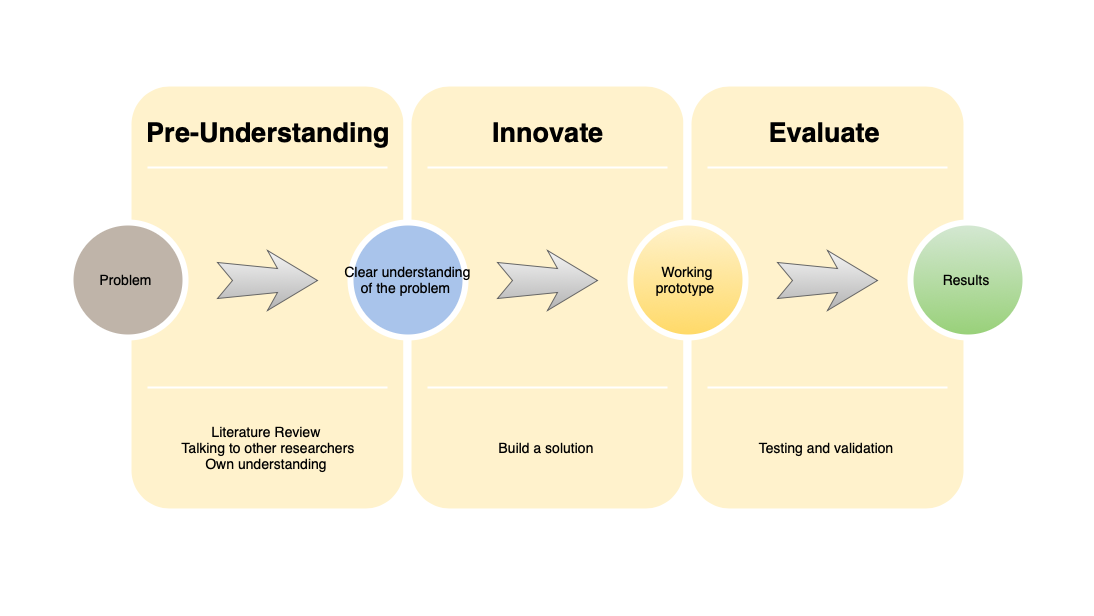
\includegraphics[scale=0.4]{constructive_approch.png}
    \caption{Flow of the Constructive Research Design }
    \label{fig:pca_w_WW_coeff_z}
\end{figure}
\vspace{12pt}

By doing so we have gained a good understanding regarding the mobile ad-hoc networking. It helped me to develop a well-rounded picture of how to implement an ad-hoc network. we came up with a new solution for Android Ad hoc networking using the readily available WIFI Direct protocol and VPN technology.

\vspace{12pt}

The next imminent problem we faced was on how to integrate the ad-hoc data plane with the cellular control plane. we were not able to find any useful resources regarding this question by doing literature reviews. So we talked with the professionals in the field to get their point of view on this problem.

\vspace{12pt}


By discussing with these people it occurred to me that to solve this solution we need a good networking toolkit and a thorough understanding of the architecture of the Android OS and Kernel.


\vspace{12pt}

So to create a good toolkit it was obvious to me that we need to port the Linux pkg manager to the Android.  This was done using the Termux repository. Superuser privileges were needed to run those tools inside the Android kernel. So for the process of rooting the Android Nexus 5x device, I found the necessary instructions in the XDA developer’s form. With help from those posts, we created the rooting script for my Nexus 5x devices.




\vspace{12pt}


By analyzing the networking implementations in the Android devices with the help of the previously mentioned tools and the Android kernel source code we were able to come up with the following architecture for this hybrid network as shown in the Figure \ref{fig:pca_coeff_z_swd}.
\clearpage
\vspace{12pt}
\begin{figure}[H]
    \centering
    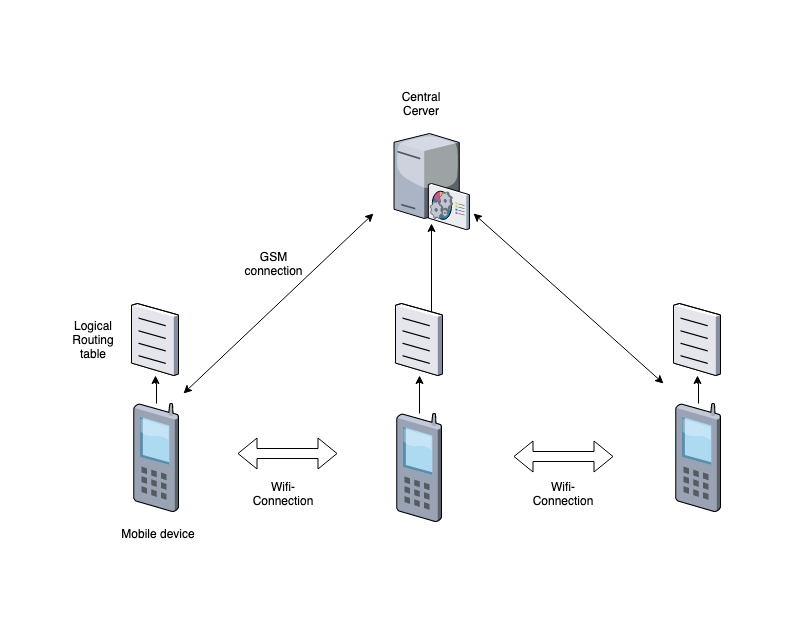
\includegraphics[scale=0.38]{network_Hiararchy}
    \caption{Network Architecture diagram }
    \label{fig:pca_coeff_z_swd}
\end{figure}


\vspace{12pt}
The first problem we faced when implementing this network architecture is that the server needs a secure way to remotely configure its end devices(Android phones). The most simple and safest way to remotely log into a Linux device is to use an SSH client. But there is a caveat, to log in to the end device first we need to know its IP address. In our case this is dynamic. So to overcome this we used reverse ssh connections. As we know the IP address of the central server every device makes a reverse ssh tunnel to that server. Then the server can use that reverse tunnel to connect to the relevant end device. 

\vspace{12pt}

A tunnel interface is created inside the ad-hoc network to make the routing between networks to become feasible. For the network switching part, we have used routing table priories rather than a demon. This is because it is a much more simple and effective solution to implement. 

\vspace{12pt}
\begin{figure}[H]
    \centering
    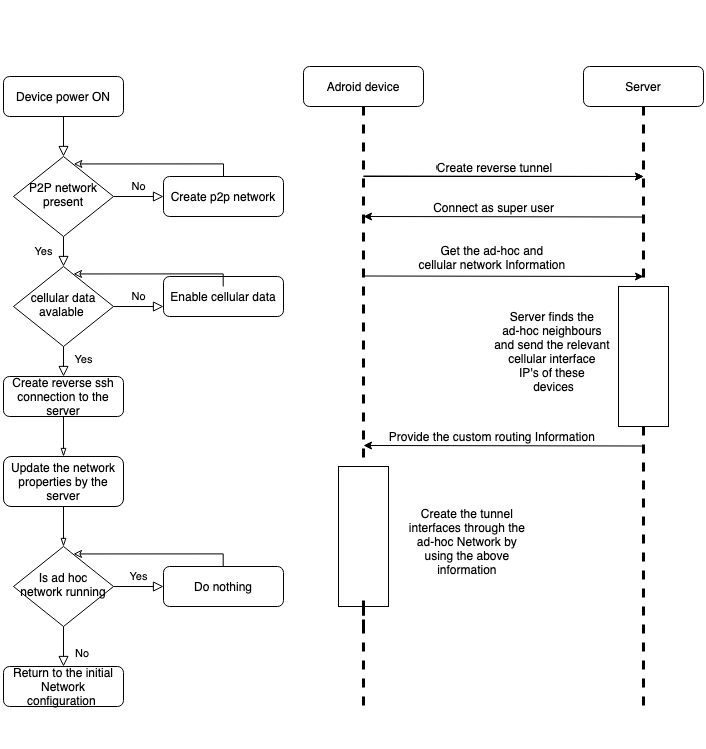
\includegraphics[scale=0.55]{flowchart2}
    \caption{Flow diagram and activity diagram for the control plane}
    \label{fig:pca_coeff_z_1121}
\end{figure}
\vspace{12pt}

We need to analyze the ad-hoc network using relevant benchmarks in this field. To identify relevant benchmark metrics we have used the above literature review. we have identified Throughput, Topology construction time, Latency as valid matrices for this evaluation process. Finally, by using these data we can predict the performance of different applications on this network. To evaluate the control plane switching, we have used the switching time as an evaluation matrix.

\vspace{12pt}
\clearpage







